% ~~~~~~~~~~~~~~~~~~~~~~~~~~~~~~~~~~~~~~~~~~~~~~~~~
\newpage
\section[Beispiele]{Beispiele}
\label{sec:Beispiele}
% ~~~~~~~~~~~~~~~~~~~~~~~~~~~~~~~~~~~~~~~~~~~~~~~~~
%
In den folgenden Abschnitten kommen ein paar grundlegende Beispiele zur Anwendung der Vorlage.
Am besten vom Beispiel im Vorschaufenster direkt in den Code springen um zu sehen wie das Beispiel umgesetzt wird.\\
Aufwendigere Beispiele sind in 01-Content/SampleFiles/Anwendungsbeispiele.tex.
Was man da nicht findet, findet man in der Overleaf Dokumentation \url{https://www.overleaf.com/learn}.
%
%
%
% ~ ~ ~ ~ ~ ~ ~ ~ ~ ~ ~ ~ ~ ~ ~ ~ ~ ~ ~ ~ ~ ~ ~ ~ ~ 
\subsection{Abbildung}
\label{sec:Beispiele_Abbildung}
% ~ ~ ~ ~ ~ ~ ~ ~ ~ ~ ~ ~ ~ ~ ~ ~ ~ ~ ~ ~ ~ ~ ~ ~ ~ 
%
Abbildungen werden in der figure-Umgebung gesetzt.
Die caption (Beschriftung) wird nach dem Code zum Bild einfügen gesetzt.
Zusätzlich kann ein Label für Querverweise vergeben werden. Abbildung \ref{fig:SampleFig} ist ein Beispiel.
%
\begin{figure}[bht]
    \centering
    \includegraphics[width=0.6\linewidth]{\GraficPath Logo-THRo}
    \caption{Das ist unser TH logo}
    \label{fig:SampleFig}
\end{figure}
%
\par
Die Größe des Bildes kann im Befehl
\begin{lstlisting}[language=tex]
\includegraphics[width=0.6\linewidth]{\GraficPath Logo-THRo}
\end{lstlisting}
in den eckigen Klammern definiert werden.
Hier ist es empfehlenswert die breite relativ zur Textbreite (textwidth, linewidth oder columnwidth) zu setzen und keine absoluten Maße zu verwenden.
%
%
%
% ~ ~ ~ ~ ~ ~ ~ ~ ~ ~ ~ ~ ~ ~ ~ ~ ~ ~ ~ ~ ~ ~ ~ ~ ~ 
\subsection{Tabellen}
\label{sec:Beispiele_Tabelle}
% ~ ~ ~ ~ ~ ~ ~ ~ ~ ~ ~ ~ ~ ~ ~ ~ ~ ~ ~ ~ ~ ~ ~ ~ ~ 
%
Tabellen werden in der table-Umgebung gesetzt.
Dabei ist zu beachten, dass die caption (Beschriftung) oberhalb positioniert werden soll.
Wie bei Abbildungen kann ein Label für Querverweise gesetzt werden.
%
\begin{table}[htb]
	\centering
	\caption{Normale Tabelle mit dem booktabs Stil}
	\label{tab:SampleTable}
	\begin{tabular}{@{}lllll@{}}
		\toprule
		& A & B  & C  & D  \\ \midrule
		a & 1 & 2  & 3  & 4  \\
		b & 5 & 6  & 7  & 8  \\
		c & 9 & 10 & 11 & 12 \\ \bottomrule
	\end{tabular}
\end{table}
%
\begin{table}[htb]
 	\centering
    \caption{Tabelle im booktabs Stil mit Fußnoten}
 	\label{tab:anytab}
 	\begin{threeparttable}
 		%
 		%
 		\begin{tabular}{@{}lllll@{}}
		\toprule
		& A & B  & C  & D  \\ \midrule
		a & 1 & 2  & 3  & 4  \\
		b & 5\tnote{a} & 6  & 7  & 8  \\
		c & 9 & 10 & 11 & 12\tnote{b} \\ \bottomrule
	    \end{tabular}
 		%
 		\begin{tablenotes}
 			\item[a]	\footnotesize	bla
 			\item[b]	\footnotesize	blabla
 		\end{tablenotes}
 		%
 	\end{threeparttable}
 \end{table}
%
%
%
% ~ ~ ~ ~ ~ ~ ~ ~ ~ ~ ~ ~ ~ ~ ~ ~ ~ ~ ~ ~ ~ ~ ~ ~ ~ 
\subsection{Symbole und Abkürzungen}
\label{sec:Beispiele_SymboleAbk}
% ~ ~ ~ ~ ~ ~ ~ ~ ~ ~ ~ ~ ~ ~ ~ ~ ~ ~ ~ ~ ~ ~ ~ ~ ~ 
%
Symbole und Abkürzungen werden im Symbol- und Abkürzungsverzeichnis in den Dateien \textbf{Symbols.tex} bzw. \textbf{Abbreviations.tex} im Ordner \textbf{13-Frontmatter} definiert.
Im Fließtext oder in Formeln werden sie folgenderweise eingebunden:
%
%
%
% ~   ~   ~   ~   ~   ~   ~   ~   ~   ~   ~   ~   ~
\subsubsection{Abkürzungen}
\label{sec:Beispiele_SymboleAbk_Abk}
% ~   ~   ~   ~   ~   ~   ~   ~   ~   ~   ~   ~   ~
%
\begin{lstlisting}[language=tex]
\ac{FRF}
\end{lstlisting}
gibt beim ersten Auftauchen im Dokument: \ac{FRF}, also den vollen Begriff mit der Abkürzung in Klammern.
Und beim zweiten mal \ac{FRF}, also nur noch die Abkürzung.\\
%
\begin{lstlisting}[language=tex]
\acf{FRF}
\end{lstlisting}
gibt immer den vollen Begriff mit der Abkürzung in Klammern: \acf{FRF}\\
%
\begin{lstlisting}[language=tex]
\acs{FRF}
\end{lstlisting}
gibt immer nur die Abkürzung: \acs{FRF}\\
%
\begin{lstlisting}[language=tex]
\acp{FRF}
\end{lstlisting}
gibt die Pluralform: \acp{FRF} 
%
%
% ~   ~   ~   ~   ~   ~   ~   ~   ~   ~   ~   ~   ~
\subsubsection{Symbole}
\label{sec:Beispiele_SymboleAbk_Symbole}
% ~   ~   ~   ~   ~   ~   ~   ~   ~   ~   ~   ~   ~
%
Das ganze funktioniert analog für die Symbole.
Wobei hier nur der Befehl
%
\begin{lstlisting}[language=tex]
\acs{<Abk. aus Symbolverzeichnis>}
\end{lstlisting}
relevant ist.
Beispiel:
\begin{lstlisting}[language=tex]
\acs{c}\acs{subAir}
\end{lstlisting}
gibt: \acs{c}\acs{subAir}
\par
Sollten Symbole benötigt werden, die noch nicht in der Datei \textbf{Symbols.tex} enthalten sind, können diese ergänzt werden.
Dabei am besten den Codeblock eines Symbols kopieren und nach den eigenen Bedürfnissen anpassen.
Beim Erstellen neuer eigener Symbole sollten aber die \textbf{Schreibregeln nach \citeauthor{DINENISO800001:201308}, Abschnitt 7} beachtet werden.
%
%
%
% ~   ~   ~   ~   ~   ~   ~   ~   ~   ~   ~   ~   ~
\subsubsection{Symbole: Wichtig zu beachten!}
\label{sec:Beispiele_SymboleAbk_Beachten}
% ~   ~   ~   ~   ~   ~   ~   ~   ~   ~   ~   ~   ~
%
Das Symbolverzeichnis besteht aus drei Abschnitten:
\begin{itemize}
    \item Lateinische Buchstaben (unterteilt in Groß- und Kleinbuchstaben)
    \item Griechische Buchstaben (unterteilt in Groß- und Kleinbuchstaben)
    \item Tiefstellungen
\end{itemize}
Werden aus einem der drei Abschnitte keine Symbole im Dokument verwendet, dann muss dieser Abschnitt in von der Markierung
%
\begin{lstlisting}[language=tex]
% -----------------------------------------------------
% >>>> A N F A N G 
\end{lstlisting}
%
bis zur Markierung
%
\begin{lstlisting}[language=tex]
% >>>> E N D E
% -----------------------------------------------------
\end{lstlisting}
%
auskommentiert werden.
Sonst erscheint die Fehlermeldung in Abbildung~\ref{fig:MissingItemFehler}.
%
\begin{figure}[htb]
    \centering
    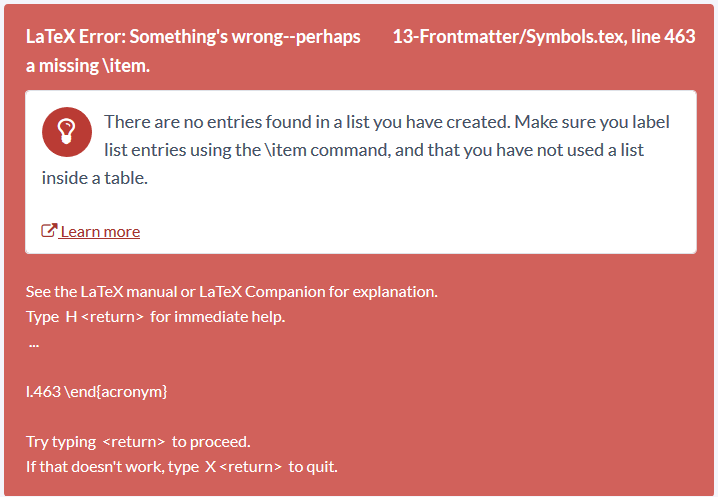
\includegraphics[width=0.6\linewidth]{\GraficPath SampleFigs/MissingItemFehler}
    \caption{Fehlermeldung in Overleaf: missing \textbackslash item}
    \label{fig:MissingItemFehler}
\end{figure}
%
Damit die Vorlage läuft, wird an dieser Stelle nun aus jedem Abschnitt ein Symbol eingefügt.
\acs{A} \acs{alpha} \acs{subAir}
%
%
%
% ~   ~   ~   ~   ~   ~   ~   ~   ~   ~   ~   ~   ~
\subsubsection{Symbole: Mathematische Operatoren}
\label{sec:Beispiele_SymboleAbk_MathOp}
% ~   ~   ~   ~   ~   ~   ~   ~   ~   ~   ~   ~   ~
%
Optional kann im Symbolverzeichnis (\textbf{Symbols.tex}) auch ein Abschnitt mit mathematischen Operatoren aufgeführt werden.
Diese werden nur im Symbolverzeichnis aufgelistet.
Ein Abruf im Dokument wie bei Abkürzungen oder Symbolen ist nicht angedacht und auch nicht möglich.
In der Datei \textbf{Symbols.tex} sind ein paar Beispiele enthalten.
\par
Falls der Abschnitt der mathematischen Operatoren nicht gebraucht wird, einfach den Codeblock von der Markierung
%
\begin{lstlisting}[language=tex]
% -----------------------------------------------------
% >>>> A N F A N G 
%
% M A T H.   O P E R A T O R E N
\end{lstlisting}
%
bis zur Markierung
%
\begin{lstlisting}[language=tex]
% M A T H.   O P E R A T O R E N
%
% >>>> E N D E
% -----------------------------------------------------
\end{lstlisting}
%
auskommentieren.
%
%
%
%
%
% ~ ~ ~ ~ ~ ~ ~ ~ ~ ~ ~ ~ ~ ~ ~ ~ ~ ~ ~ ~ ~ ~ ~ ~ ~ 
\subsection{Formeln}
\label{sec:Beispiele_Formeln}
% ~ ~ ~ ~ ~ ~ ~ ~ ~ ~ ~ ~ ~ ~ ~ ~ ~ ~ ~ ~ ~ ~ ~ ~ ~ 
%
Werden in der euquation-Umgebung gesetzt.
Dabei können sie auch mit einem Label für Querverweise versehen werden.
Für Querverweise auf Formeln folgenden Befehl verwenden.
\begin{lstlisting}[language=tex]
\eqref{<label>}
\end{lstlisting}
%
Damit wird die Zahl in runde Klammern gesetzt \eqref{eq:Ekin}.
\par
Hinweis: Auch in der Formelumgebung können die Symbole wie in Abschnitt \ref{sec:Beispiele_SymboleAbk_Abk} beschrieben verwendet werden.
\par
Beispiel:
%
\begin{lstlisting}[language=tex]
\begin{equation}
    \acs{Ek} = \frac{1}{2} \acs{m} \acs{v}^2
    \label{eq:Ekin}
\end{equation}
\end{lstlisting}
%
\begin{equation}
    \acs{Ek} = \frac{1}{2} \acs{m} \acs{v}^2
    \label{eq:Ekin}
\end{equation}
%
%
%
% ~ ~ ~ ~ ~ ~ ~ ~ ~ ~ ~ ~ ~ ~ ~ ~ ~ ~ ~ ~ ~ ~ ~ ~ ~ 
\subsection{Einheiten und Zahlen im Text}
\label{sec:Beispiele_EinheitenZahlen}
% ~ ~ ~ ~ ~ ~ ~ ~ ~ ~ ~ ~ ~ ~ ~ ~ ~ ~ ~ ~ ~ ~ ~ ~ ~ 
%
Einheiten und Zahlen im Text und in Formeln mit den folgenden Befehlen setzen
(siehe auch \url{https://ctan.net/macros/latex/contrib/siunitx/siunitx.pdf}):
%
\begin{itemize}
    \item 
\begin{lstlisting}[language=tex]
\si{\metre \per \square \second}
\end{lstlisting}
gibt: \si{\metre \per \square \second}\\
%
    \item 
\begin{lstlisting}[language=tex]
\SI{e-2}{\metre\per\newton\per\second}
\end{lstlisting}
gibt: \SI{e-2}{\metre\per\newton\per\second}\\
%
    \item 
\begin{lstlisting}[language=tex]
\SIrange{2.5e-4}{1.2e-2}{\metre\per\newton\per\second}
\end{lstlisting}
gibt: \SIrange{2.5e-4}{1.2e-2}{\metre\per\newton\per\second}\\
%
    \item 
\begin{lstlisting}[language=tex]
\num{2e-5}
\end{lstlisting}
gibt: \num{2e-5}
\end{itemize}
%
%
%
%
% ~ ~ ~ ~ ~ ~ ~ ~ ~ ~ ~ ~ ~ ~ ~ ~ ~ ~ ~ ~ ~ ~ ~ ~ ~ 
\subsection{Bezug auf Abschnitte, Gleichungen, Abbildungen und Tabellen}
\label{sec:Beispiele_Referenz}
% ~ ~ ~ ~ ~ ~ ~ ~ ~ ~ ~ ~ ~ ~ ~ ~ ~ ~ ~ ~ ~ ~ ~ ~ ~ 
%
Um auf Abschnitte, Abbildungen und Tabellen zu verweisen wird der Befehl
%
\begin{lstlisting}[language=tex]
\ref{<Labelname>}
\end{lstlisting}
%
verwendet.
\par
Beispiel:
\begin{lstlisting}[language=tex]
In Abschnitt~\ref{sec:Beispiele_Abbildung} ist 
Abbildung~\ref{fig:SampleFig} gezeigt.
\end{lstlisting}
In Abschnitt~\ref{sec:Beispiele_Abbildung} ist Abbildung~\ref{fig:SampleFig} gezeigt.
\par
Die Tilde verhindert einen Zeilenumbruch vor der Nummer.
%
%
%
% ~ ~ ~ ~ ~ ~ ~ ~ ~ ~ ~ ~ ~ ~ ~ ~ ~ ~ ~ ~ ~ ~ ~ ~ ~ 
\subsection{Zitierbefehle}
\label{sec:Beispiele_Zitierbefehle}
% ~ ~ ~ ~ ~ ~ ~ ~ ~ ~ ~ ~ ~ ~ ~ ~ ~ ~ ~ ~ ~ ~ ~ ~ ~ 
%
Zum Zitieren muss ein Eintrag in der Datei Literatur.bib hinterlegt sein.
Dieser kann zum Beispiel über einen bibtex-Export direkt aus Citavi erzeugt werden.
\par
Der sogenannte BibTeX Key wird zum zitieren verwendet.
%
\begin{lstlisting}[language=tex]
\cite{<BibTeX Key>}
\end{lstlisting}
%
Folgende Varianten sind zum zitieren im Text möglich:
%
\begin{itemize}
    \item 
\begin{lstlisting}[language=tex]
\cite{Cremer.1967}
\end{lstlisting}
gibt: \cite{Cremer.1967}\\
%
    \item 
\begin{lstlisting}[language=tex]
\textcite{Cremer.1967}
\end{lstlisting}
gibt: \textcite{Cremer.1967}\\
%
    \item 
\begin{lstlisting}[language=tex]
\citeauthor{Cremer.1967}
\end{lstlisting}
gibt: \citeauthor{Cremer.1967}\\
%
    \item 
\begin{lstlisting}[language=tex]
\parencite{Cremer.1967}
\end{lstlisting}
gibt: \parencite{Cremer.1967}\\
%
    \item 
\begin{lstlisting}[language=tex]
\parencite*{Cremer.1967}
\end{lstlisting}
gibt: \parencite*{Cremer.1967}\\
%
\end{itemize}
%
\par
Zusätzlich können Seitenzahl oder Ähnliches angehängt werden:
\begin{itemize}
    \item 
\begin{lstlisting}[language=tex]
\textcite[\pno~59]{Cremer.1967}
\end{lstlisting}
gibt:  \textcite[\pno~59]{Cremer.1967}\\
%
    \item 
\begin{lstlisting}[language=tex]
\parencite[see][59--63]{Cremer.1967}
\end{lstlisting} 
\parencite[see][59--63]{Cremer.1967}\\
%
\end{itemize}
\par
\textbf{Beim zitieren von Normen beachten:}\\
Ausschließlich(!) mit 
\begin{lstlisting}[language=tex]
\citeauthor{}
\end{lstlisting}
zitieren, da hier die Jahreszahl schon beim Autor dabei steht. Beispiel:
\citeauthor{DINENISO800001:201308}.
Der entsprechende bibtex Eintrag sieht so aus:
\begin{lstlisting}[language=tex]
@misc{DINENISO800001:201308,
 author = {{DIN EN ISO 80000-1:2013-08}},
 title = {Gr{\"o}{\ss}en und Einheiten: Teil 1: Allgemeines}
}
\end{lstlisting}
%
%
%
% ~ ~ ~ ~ ~ ~ ~ ~ ~ ~ ~ ~ ~ ~ ~ ~ ~ ~ ~ ~ ~ ~ ~ ~ ~ 
\subsection{Todo notes}
\label{sec:ToDoNotes}
% ~ ~ ~ ~ ~ ~ ~ ~ ~ ~ ~ ~ ~ ~ ~ ~ ~ ~ ~ ~ ~ ~ ~ ~ ~ 
%
(siehe auch \url{https://ctan.mc1.root.project-creative.net/macros/latex/contrib/todonotes/todonotes.pdf})
%
\par
Dieses Paket ist sehr nützlich um sich im Dokument todo Notizen zu setzen.
Die Notiz kann entweder am Seitenrand
\todo{Hier muss ich noch eine Literaturstelle nachschauen.}
oder direkt im Text plaziert werden
\todo[inline]{ToDo Notiz in der Zeile}
\par
Mit dem Befehl
\begin{lstlisting}[language=tex]
\listoftodos
\end{lstlisting} 
kann ein an jeder beliebigen Stelle ein Verzeichnis der eingefügten todos angelegt werden.
Siehe nächste Seite:
\listoftodos